\chapter{Simulator GUI}\label{sec:simulator_pictures}
\begin{figure}[H]
    \centering
   	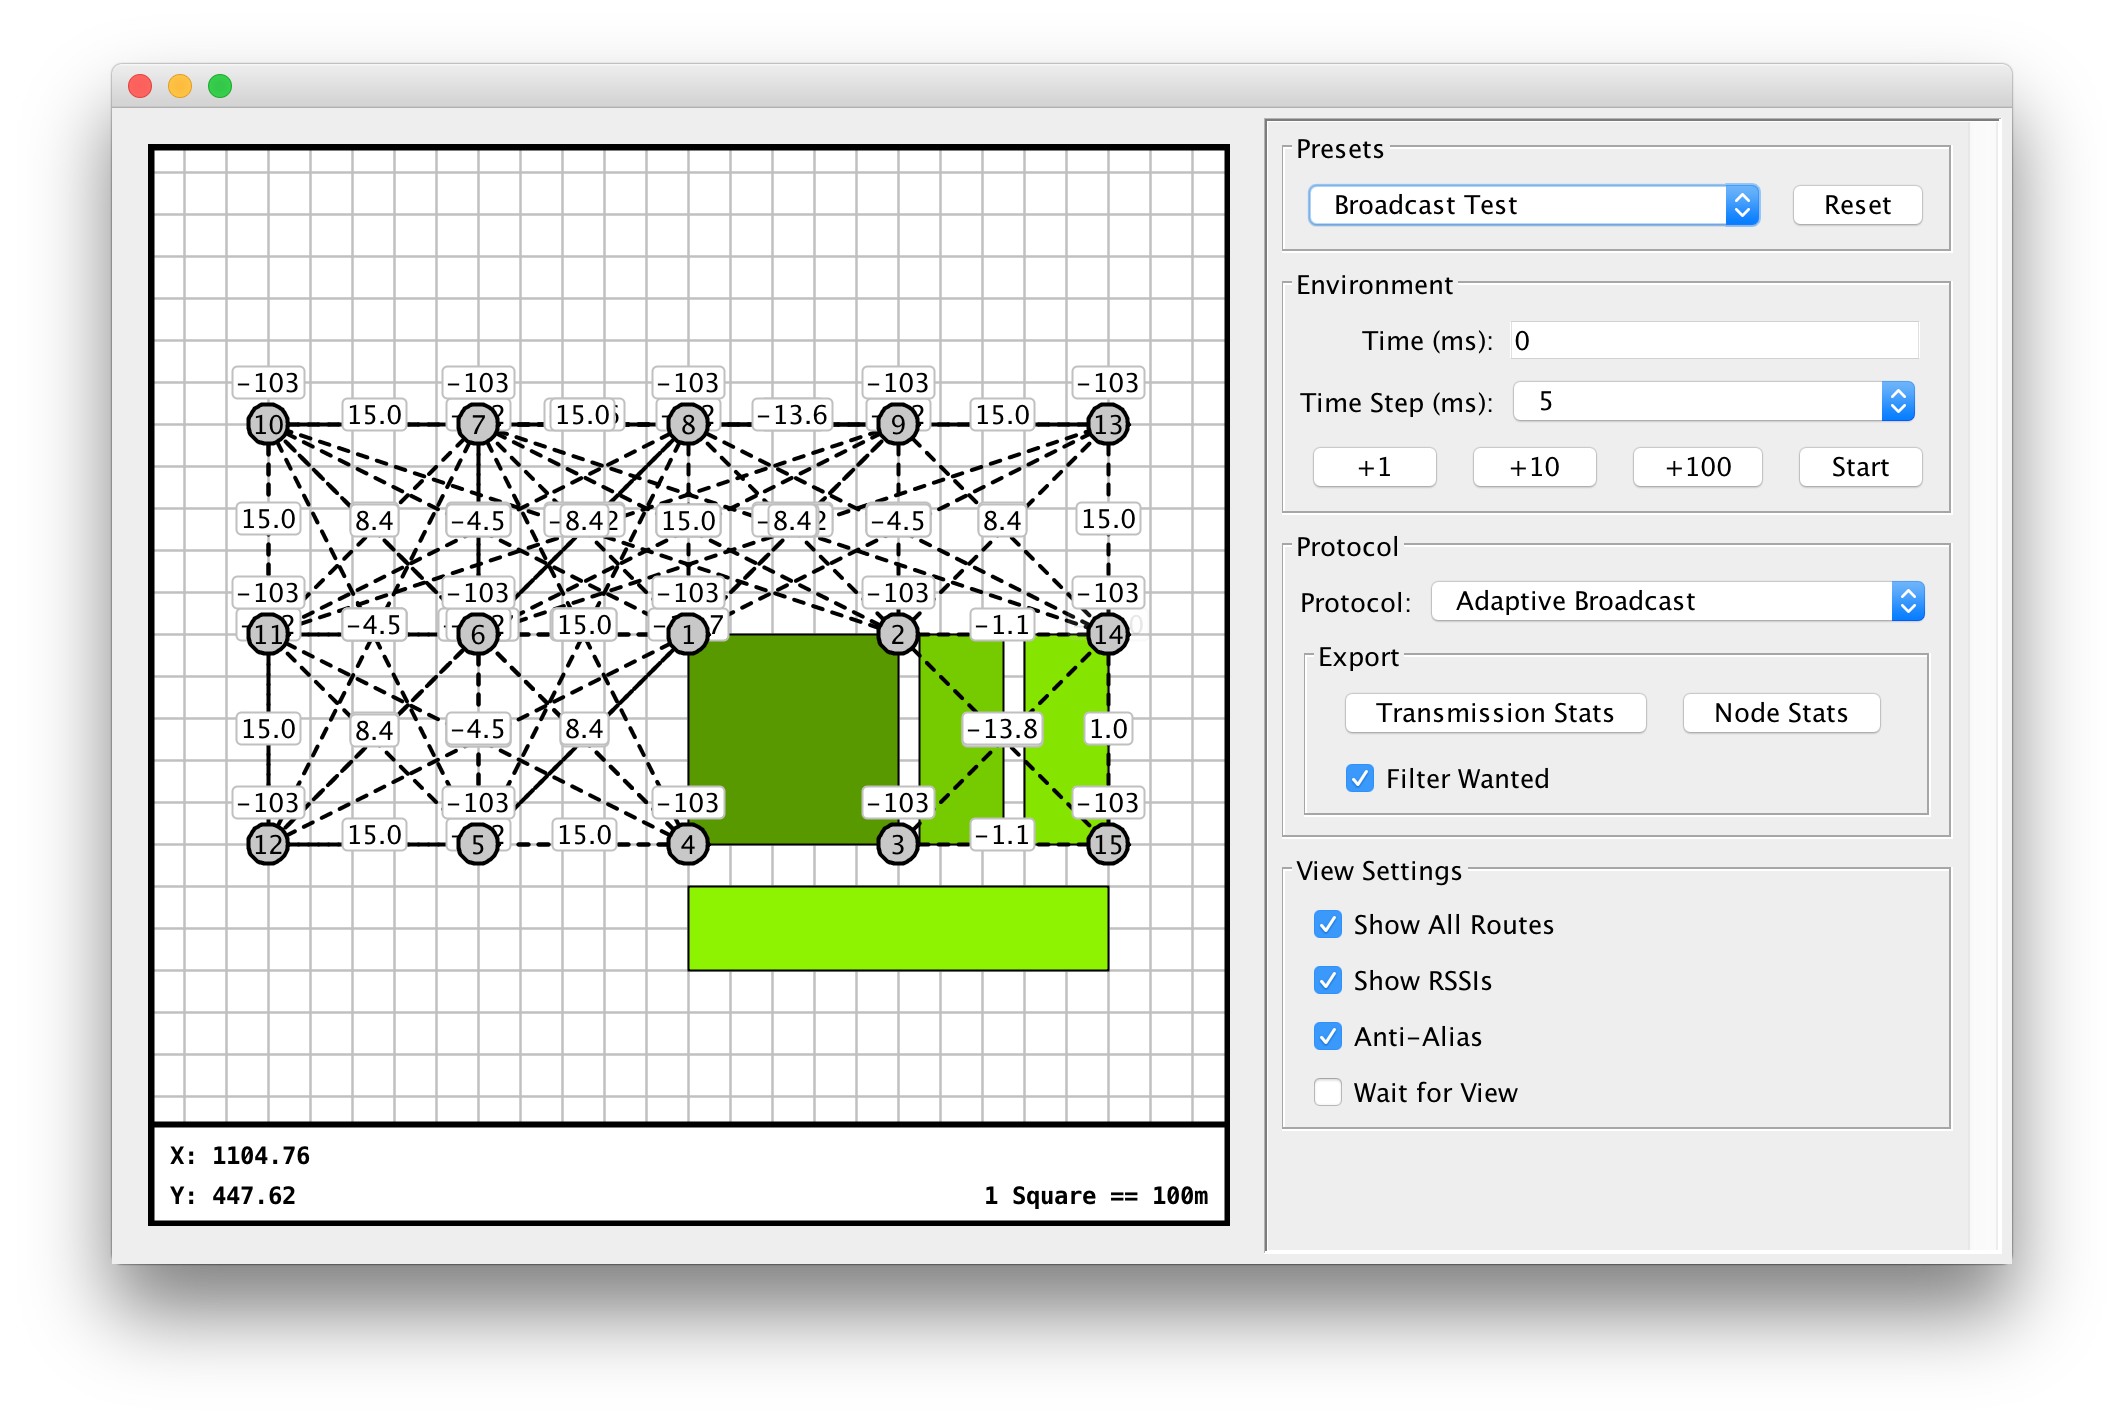
\includegraphics[width=\textwidth]{Figures/simulator_all_routes}
    \caption[Simulator view with all routes shown]{
    	Simulator view when all potential receivable routes are being shown. No transmissions are actually occurring.
    }
\end{figure}

\begin{figure}[H]
    \centering
   	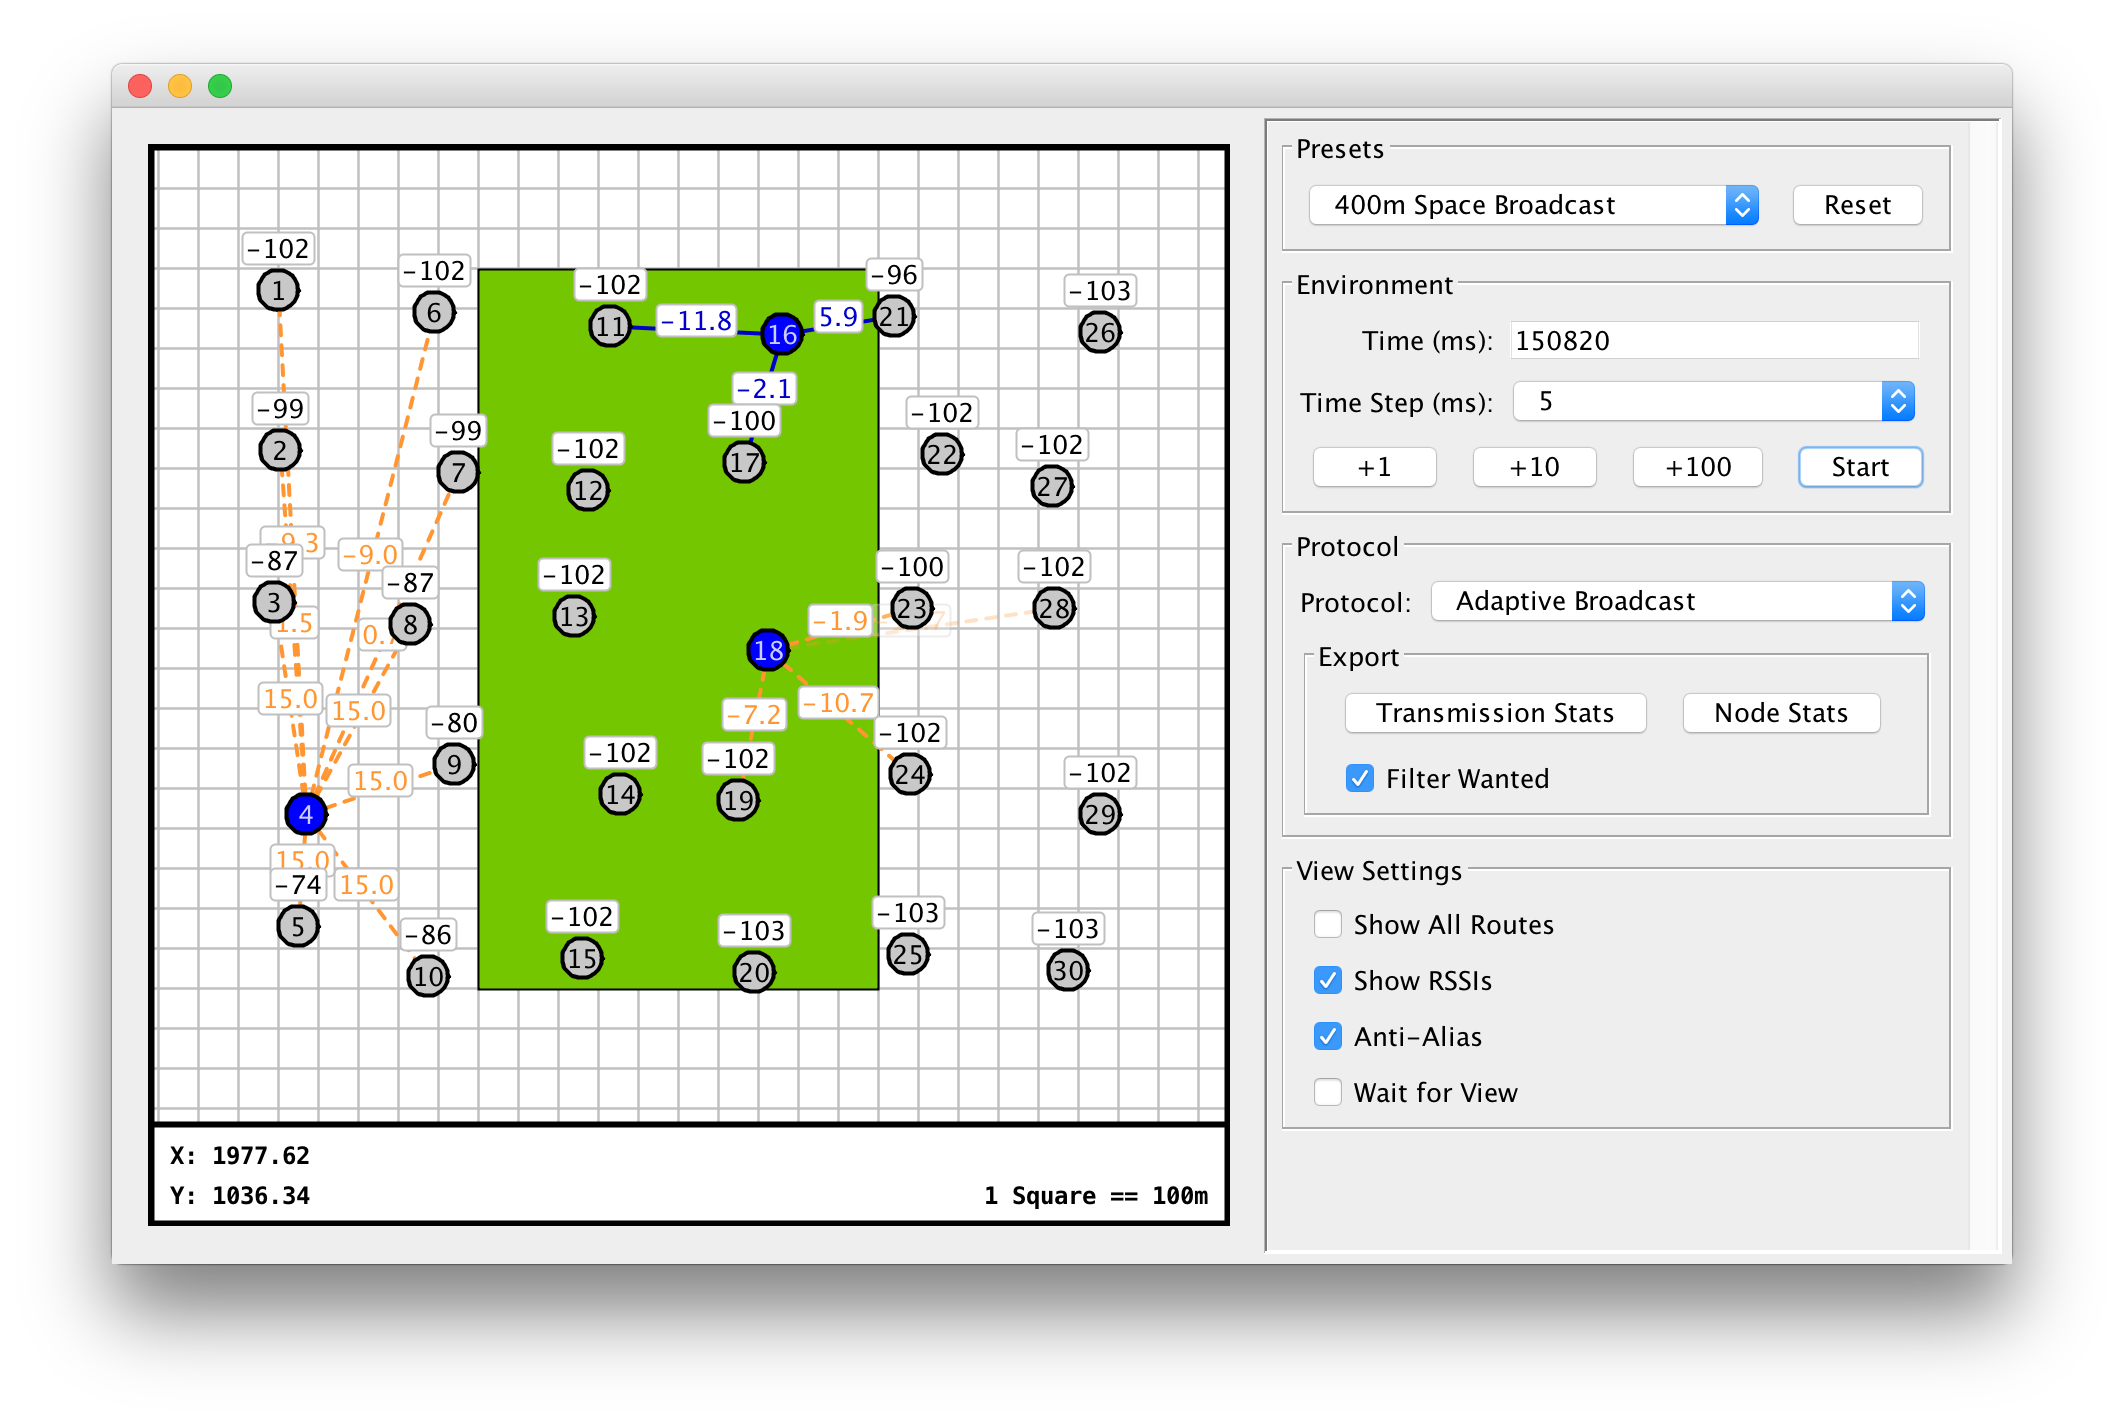
\includegraphics[width=\textwidth]{Figures/simulator_overhead}
    \caption[Simulator view with data and overhead]{
    	Simulator view when some transmissions are protocol overhead packets, whilst others are data packets.
    }
\end{figure}

\begin{figure}[H]
    \centering
   	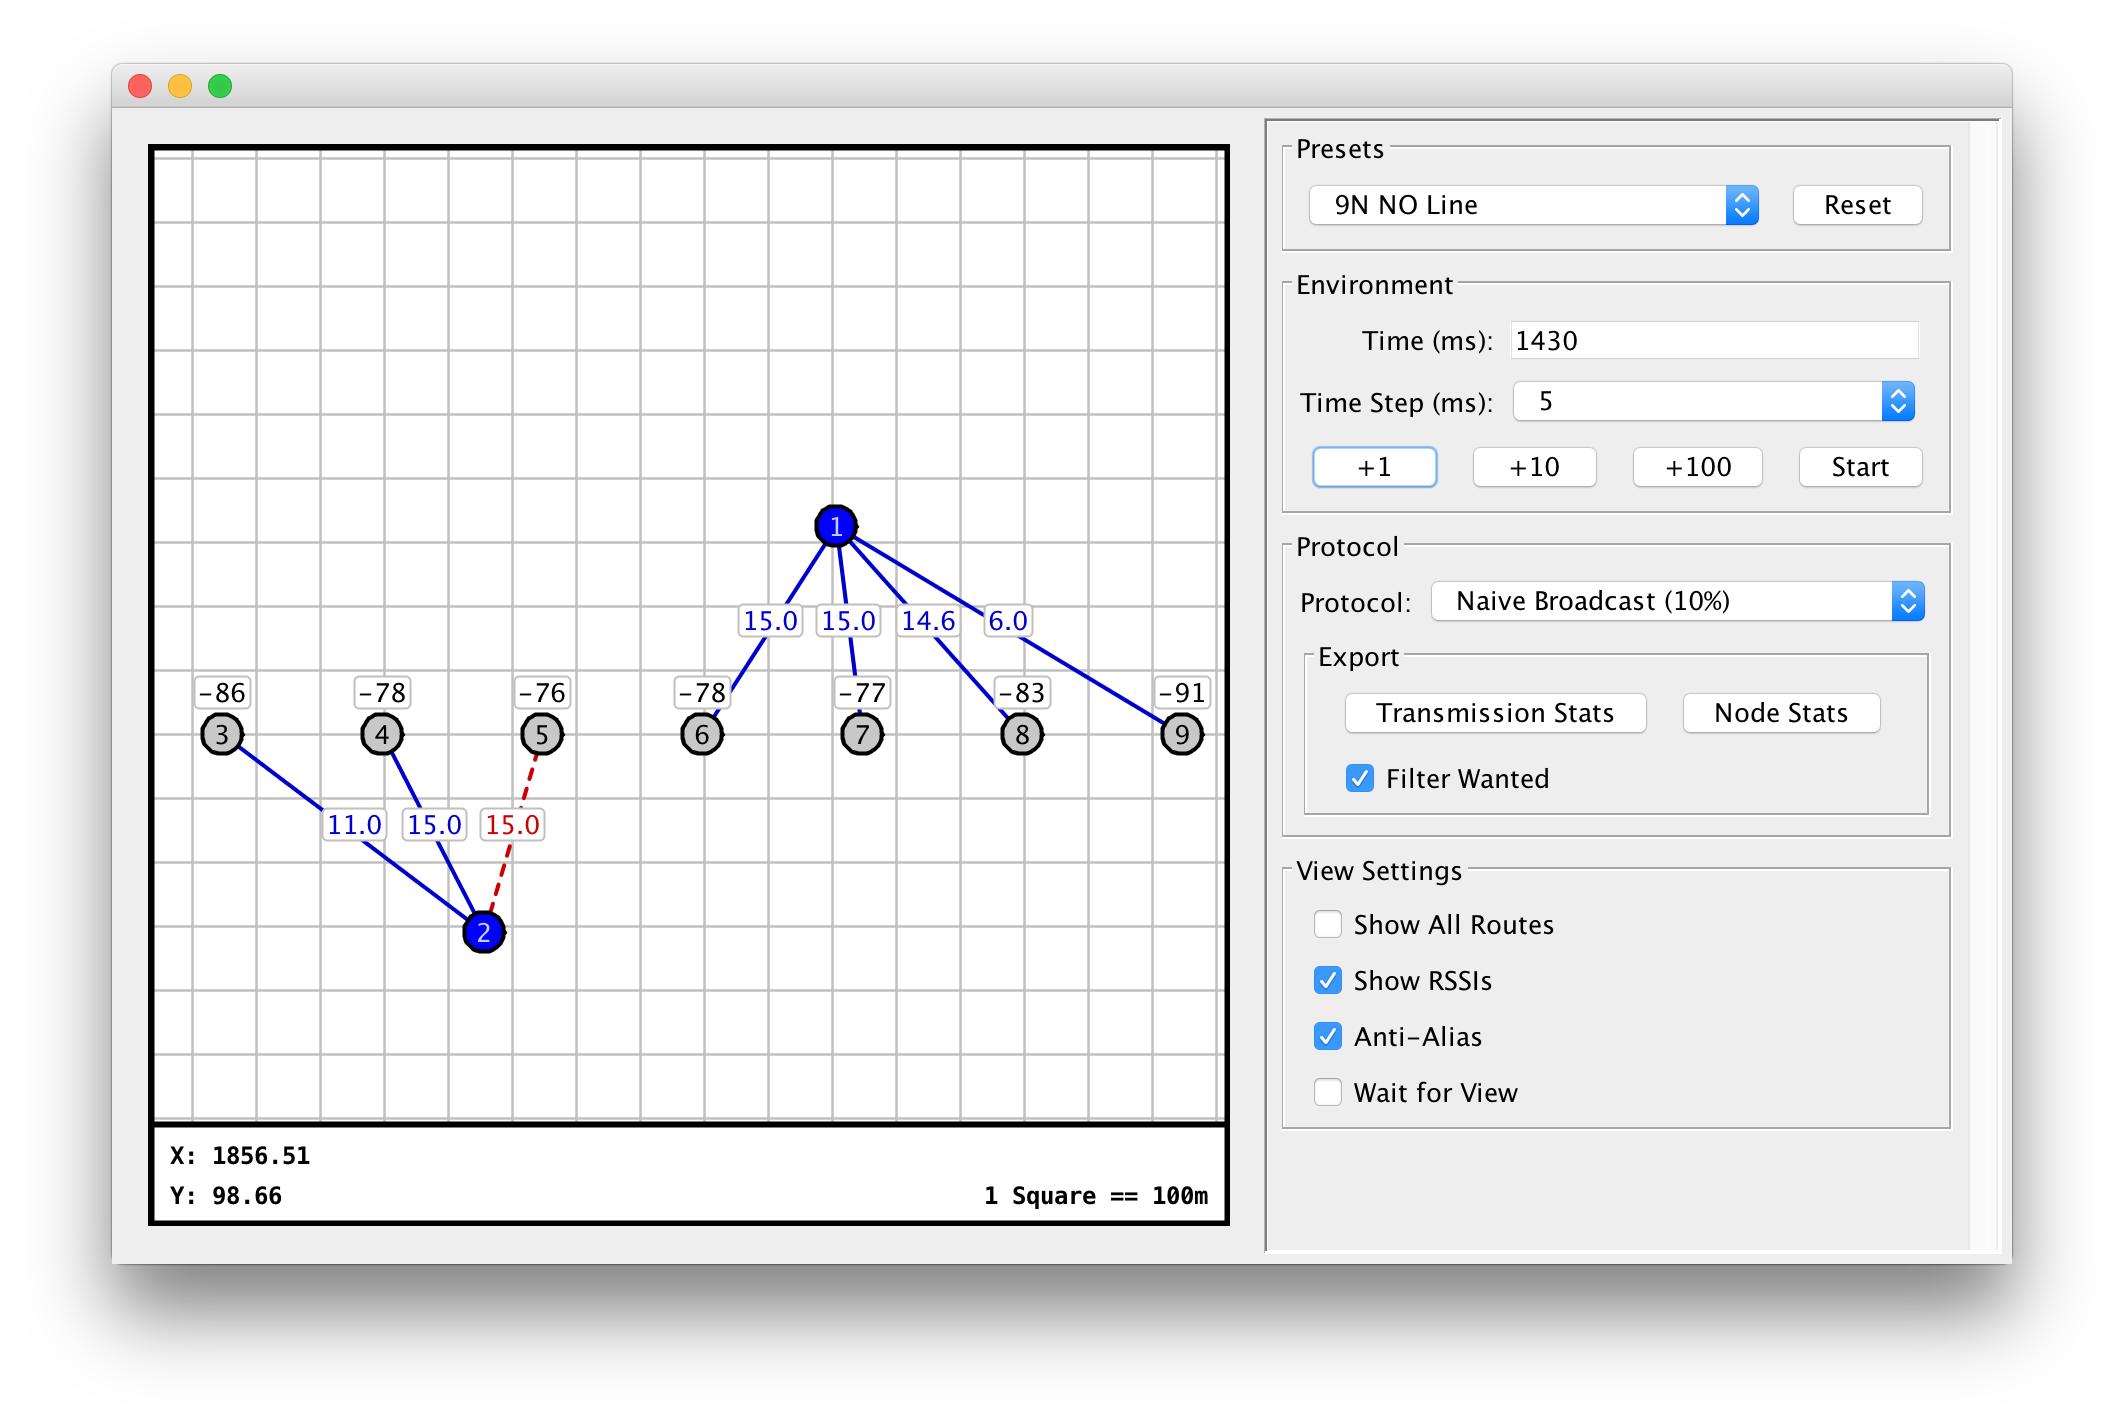
\includegraphics[width=\textwidth]{Figures/simulator_interference}
    \caption[Simulator view with interference]{
    	Simulator view when a stronger transmission (from 2) has started after a receiver (5) has already synchronised with a transmission (from 1).
    }
\end{figure}
